
%% bare_conf.tex
%% V1.4b
%% 2015/08/26
%% by Michael Shell
%% See:
%% http://www.michaelshell.org/
%% for current contact information.
%%
%% This is a skeleton file demonstrating the use of IEEEtran.cls
%% (requires IEEEtran.cls version 1.8b or later) with an IEEE
%% conference paper.
%%
%% Support sites:
%% http://www.michaelshell.org/tex/ieeetran/
%% http://www.ctan.org/pkg/ieeetran
%% and
%% http://www.ieee.org/

%%*************************************************************************
%% Legal Notice:
%% This code is offered as-is without any warranty either expressed or
%% implied; without even the implied warranty of MERCHANTABILITY or
%% FITNESS FOR A PARTICULAR PURPOSE! 
%% User assumes all risk.
%% In no event shall the IEEE or any contributor to this code be liable for
%% any damages or losses, including, but not limited to, incidental,
%% consequential, or any other damages, resulting from the use or misuse
%% of any information contained here.
%%
%% All comments are the opinions of their respective authors and are not
%% necessarily endorsed by the IEEE.
%%
%% This work is distributed under the LaTeX Project Public License (LPPL)
%% ( http://www.latex-project.org/ ) version 1.3, and may be freely used,
%% distributed and modified. A copy of the LPPL, version 1.3, is included
%% in the base LaTeX documentation of all distributions of LaTeX released
%% 2003/12/01 or later.
%% Retain all contribution notices and credits.
%% ** Modified files should be clearly indicated as such, including  **
%% ** renaming them and changing author support contact information. **
%%*************************************************************************


% *** Authors should verify (and, if needed, correct) their LaTeX system  ***
% *** with the testflow diagnostic prior to trusting their LaTeX platform ***
% *** with production work. The IEEE's font choices and paper sizes can   ***
% *** trigger bugs that do not appear when using other class files.       ***                          ***
% The testflow support page is at:
% http://www.michaelshell.org/tex/testflow/

\documentclass[12pt,twoside,a4paper,openright]{report}
\usepackage{etex}
% Select encoding of your inputs.
\usepackage[utf8]{inputenc}

% Make latex understand and use the typographic
% rules of the language used in the document.
\usepackage[english, danish]{babel}

% Use the vector font Latin Modern which is going
% to be the default font in latex in the future.
\usepackage{lmodern}

% Choose the font encoding
\usepackage[T1]{fontenc}

% Use colour in tables
\usepackage[table]{xcolor}
\usepackage{array}
\usepackage{multirow}

% load a colour package
\usepackage{xcolor}
\definecolor{aaublue}{RGB}{33,26,82}% dark blue

% The standard graphics inclusion package
\definecolor{white}{RGB}{255,255,255} % define color white
\usepackage{graphicx}
\usepackage{adjustbox}

% Set up how figure and table captions are displayed
\usepackage{caption}
\captionsetup{
  font=footnotesize,% set font size to footnotesize
  labelfont=bf % bold label (e.g., Figure 3.2) font
}

% Enable row combination in tables
\usepackage{multirow}

% Make space between table lines and text
\renewcommand{\arraystretch}{1.5}

% Make the standard latex tables look so much better
\usepackage{array,booktabs}

% Enable the use of frames around, e.g., theorems
% The framed package is used in the example environment
\usepackage{framed}
\usepackage{colortbl}
\usepackage{longtable}
\usepackage{xcolor}
\usepackage{textcomp}

%%%%%%%%%%%%%%%%%%%%%%%%%%%%%%%%%%%%%%%%%%%%%%%%
% Mathematics
%%%%%%%%%%%%%%%%%%%%%%%%%%%%%%%%%%%%%%%%%%%%%%%%
% Defines new environments such as equation,
% align and split 
\usepackage{amsmath}
\usepackage{relsize}
% Adds new math symbols
\usepackage{amssymb}
% Use theorems in your document
% The ntheorem package is also used for the example environment
% When using thmmarks, amsmath must be an option as well. Otherwise \eqref doesn't work anymore.
\usepackage[framed,amsmath,thmmarks]{ntheorem}
\usepackage{cancel}

%%%%%%%%%%%%%%%%%%%%%%%%%%%%%%%%%%%%%%%%%%%%%%%%
% Page Layout
%%%%%%%%%%%%%%%%%%%%%%%%%%%%%%%%%%%%%%%%%%%%%%%%
% Change margins, papersize, etc of the document
\usepackage[
  left=25mm,% left margin on an odd page %tidligere 25mm for baade right og left
  right=25mm,% right margin on an odd page
  top=35mm,
  ]{geometry}
  
% Modify how \chapter, \section, etc. look
% The titlesec package is very configureable
\usepackage{titlesec}
\makeatletter
\def\ttl@mkchap@i#1#2#3#4#5#6#7{%
    \ttl@assign\@tempskipa#3\relax\beforetitleunit
    \vspace{\@tempskipa}%<<<<<< REMOVE THE * AFTER \vspace
    \global\@afterindenttrue
    \ifcase#5 \global\@afterindentfalse\fi
    \ttl@assign\@tempskipb#4\relax\aftertitleunit
    \ttl@topmode{\@tempskipb}{%
        \ttl@select{#6}{#1}{#2}{#7}}%
    \ttl@finmarks  % Outside the box!
    \@ifundefined{ttlp@#6}{}{\ttlp@write{#6}}}
\makeatother

\titlespacing{\chapter}{0pt}{0pt}{10pt}
\titlespacing{\section}{0pt}{0pt}{-5pt}
\titlespacing{\subsection}{0pt}{8pt}{-5pt}
\titlespacing{\subsubsection}{0pt}{6pt}{-10pt}

\titleformat*{\section}{\normalfont\Large\bfseries\color{aaublue}}
\titleformat*{\subsection}{\normalfont\large\bfseries\color{aaublue}}
\titleformat*{\subsubsection}{\normalfont\normalsize\bfseries\color{aaublue}}

\usepackage{bookmark}
\usepackage{titlesec, blindtext, color}
%\color{gray75}{gray}{0.75}
\newcommand{\hsp}{\hspace{20pt}}
\titleformat{\chapter}[hang]{\Huge\bfseries}{\thechapter\hsp\textcolor{aaublue}{|}\hsp}{0pt}{\Huge\bfseries}

% Change the headers and footers
\usepackage{fancyhdr}
\setlength{\headheight}{15pt}
\pagestyle{fancy}
\fancyhf{} %delete everything
\renewcommand{\headrulewidth}{0pt} %remove the horizontal line in the header
\fancyhead[RO,LE]{\color{aaublue}\small\nouppercase\leftmark} %even page - chapter title
\fancyhead[LO]{}
\fancyhead[RE]{} 
\fancyhead[CE]{}
\fancyhead[CO]{}
\fancyfoot[RE,LO]{\thepage}
\fancyfoot[LE,RO]{} %page number on all pages
\fancyfoot[CE,CO]{}

% change first page of all chapters header and footer to fancy style
\makeatletter
\let\ps@plain\ps@fancy
\makeatother

% Do not stretch the content of a page. Instead,
% insert white space at the bottom of the page
\raggedbottom

% Enable arithmetics with length. Useful when typesetting the layout.
\usepackage{calc}

%%%%%%%%%%%%%%%%%%%%%%%%%%%%%%%%%%%%%%%%%%%%%%%%
% Bibliography
%%%%%%%%%%%%%%%%%%%%%%%%%%%%%%%%%%%%%%%%%%%%%%%%
%setting references (using numbers) and supporting i.a. Chicargo-style:
\usepackage{etex}
\usepackage{etoolbox}
\usepackage{keyval}
\usepackage{ifthen}
\usepackage{url}
\usepackage{csquotes}
\usepackage[backend=biber, url=true, doi=true, style=numeric, sorting=none]{biblatex}
\addbibresource{setup/bibliography.bib}

%%%%%%%%%%%%%%%%%%%%%%%%%%%%%%%%%%%%%%%%%%%%%%%%
% Misc
%%%%%%%%%%%%%%%%%%%%%%%%%%%%%%%%%%%%%%%%%%%%%%%%

%%% Enables the use FiXme refferences. Syntax: \fxnote{...} %%%
\usepackage[footnote, draft, english, silent, nomargin]{fixme}
%With "final" instead of "draft" an error will ocure for every FiXme under compilation.

%%% allows use of lorem ipsum (generate i.e. pagagraph 1 to 5 with \lipsum[1-5]) %%%
\usepackage{lipsum}

%%% Enables figures with text wrapped tightly around it %%%
\usepackage{wrapfig}

%%% Section debth included in table of contents (1 = down to sections) %%%
\setcounter{tocdepth}{1}

%%% Section debth for numbers (1 = down to sections) %%%
\setcounter{secnumdepth}{1}

\usepackage{tocloft}
\setlength{\cftbeforetoctitleskip}{0 cm}
\renewcommand{\cftpartpresnum}{Part~}
\let\cftoldpartfont\cftpartfont
\renewcommand{\cftpartfont}{\cftoldpartfont\cftpartpresnum}

%%%%%%%%%%%%%%%%%%%%%%%%%%%%%%%%%%%%%%%%%%%%%%%%
% Hyperlinks
%%%%%%%%%%%%%%%%%%%%%%%%%%%%%%%%%%%%%%%%%%%%%%%%

% Enable hyperlinks and insert info into the pdf
% file. Hypperref should be loaded as one of the 
% last packages
\usepackage{nameref}
\usepackage{hyperref}
\hypersetup{%
	%pdfpagelabels=true,%
	plainpages=false,%
	pdfauthor={Author(s)},%
	pdftitle={Title},%
	pdfsubject={Subject},%
	bookmarksnumbered=true,%
	colorlinks,%
	citecolor=aaublue,%
	filecolor=aaublue,%
	linkcolor=aaublue,% you should probably change this to black before printing
	urlcolor=aaublue,%
	pdfstartview=FitH%
}

% remove all indentations
\setlength\parindent{0pt}
\parskip 5mm
\usepackage{verbatim}

\definecolor{Gra}{RGB}{230,230,230}

%creates a nice-looking C#-text
\newcommand{\CC}{C\nolinebreak\hspace{-.05em}\raisebox{.3ex}{\scriptsize\text \#} }

%enables multi column lists
\usepackage{multicol}

%enables code-examples
\usepackage{listings}

\definecolor{coolblue}{RGB}{32,95,128}
\definecolor{mygreen}{rgb}{0,0.6,0}
\definecolor{mygray}{rgb}{0.5,0.5,0.5}
\definecolor{mymauve}{rgb}{0.58,0,0.82}
\usepackage{textcomp}
\definecolor{listinggray}{gray}{0.9}
\definecolor{lbcolor}{rgb}{0.9,0.9,0.9}

\lstdefinestyle{customcpp}{
    backgroundcolor=\color{lbcolor},
    tabsize=4,
    rulecolor=,
    language=C++,
    basicstyle=\scriptsize,
    upquote=true,
    aboveskip={1.5\baselineskip},
    columns=fixed,
    showstringspaces=false,
    extendedchars=true,
    breaklines=true,
    prebreak = \raisebox{0ex}[0ex][0ex]{\ensuremath{\hookleftarrow}},
    frame=single,
    showtabs=false,
    numbers=left,
    captionpos=b,
    numbersep=5pt,
    numberstyle=\tiny\color{mygray},
    showspaces=false,
    showstringspaces=false,
    identifierstyle=\ttfamily,
    keywordstyle=\color[rgb]{0,0,1},
    commentstyle=\color[rgb]{0.133,0.545,0.133},
    stringstyle=\color[rgb]{0.627,0.126,0.941},
}
\lstdefinestyle{custommatlab}{
    backgroundcolor=\color{lbcolor},
    tabsize=4,
    rulecolor=,
    language=Matlab,
    basicstyle=\scriptsize,
    upquote=true,
    aboveskip={1.5\baselineskip},
    columns=fixed,
    showstringspaces=false,
    extendedchars=true,
    breaklines=true,
    prebreak = \raisebox{0ex}[0ex][0ex]{\ensuremath{\hookleftarrow}},
    frame=single,
    showtabs=false,
    numbers=left,
    captionpos=b,
    numbersep=5pt,
    numberstyle=\tiny\color{mygray},
    showspaces=false,
    showstringspaces=false,
    identifierstyle=\ttfamily,
    keywordstyle=\color[rgb]{0,0,1},
    commentstyle=\color[rgb]{0.133,0.545,0.133},
    stringstyle=\color[rgb]{0.627,0.126,0.941},   
}
\lstdefinestyle{custommatlabinline}{
    style=custommatlab,
    basicstyle=\small,
}
\lstdefinestyle{customcppinline}{
    style=customcpp,
    basicstyle=\small,
}
\lstset{
%  backgroundcolor=\color{white},   % choose the background color; you must add \usepackage{color} or \usepackage{xcolor}
%  basicstyle=\footnotesize,        % the size of the fonts that are used for the code
%  breakatwhitespace=false,         % sets if automatic breaks should only happen at whitespace
%  breaklines=true,                 % sets automatic line breaking
%  captionpos=t,                    % sets the caption-position to bottom
%  commentstyle=\color{mygreen},    % comment style
%  deletekeywords={...},            % if you want to delete keywords from the given language
%  escapeinside={\%*}{*)},          % if you want to add LaTeX within your code
%  extendedchars=true,              % lets you use non-ASCII characters; for 8-bits encodings only, does not work with UTF-8
%  frame=single,                    % adds a frame around the code
%  keepspaces=true,                 % keeps spaces in text, useful for keeping indentation of code (possibly needs columns=flexible)
%  keywordstyle=\color{blue},       % keyword style
%  language=C++,                 % the language of the code
%  morekeywords={*,...},            % if you want to add more keywords to the set
%  numbers=left,                    % where to put the line-numbers; possible values are (none, left, right)
%  numbersep=5pt,                   % how far the line-numbers are from the code
%  numberstyle=\tiny\color{mygray}, % the style that is used for the line-numbers
%  rulecolor=\color{black},         % if not set, the frame-color may be changed on line-breaks within not-black text (e.g. comments (green here))
%  showspaces=false,                % show spaces everywhere adding particular underscores; it overrides 'showstringspaces'
%  showstringspaces=false,          % underline spaces within strings only
%  showtabs=false,                  % show tabs within strings adding particular underscores
%  stepnumber=1,                    % the step between two line-numbers. If it's 1, each line will be numbered
%  stringstyle=\color{mymauve},     % string literal style
%  tabsize=2,                       % sets default tabsize to 2 spaces
%  title=\lstname                   % show the filename of files included with \lstinputlisting; also try caption instead of title
    style=customcpp
}

\usepackage{float}
\usepackage{caption}
\usepackage{subcaption}
\usepackage{siunitx}
\sisetup{decimalsymbol=comma}
\sisetup{detect-weight}

\usepackage{enumitem}
%\usepackage[citestyle=authoryear,natbib=true]{biblatex}

% Figures - TIKZ
\usepackage{tikz}
\usetikzlibrary{shapes,arrows}
\usepackage[americanresistors,americaninductors,americancurrents, americanvoltages]{circuitikz}

% Wall of text logo
\newcommand{\walloftextalert}[0]{\includegraphics[width=\textwidth]{walloftext.png}}

\usepackage{pdfpages}
\usepackage{lastpage}
\usepackage{epstopdf}

\setlength{\headheight}{21pt}

\hfuzz=\maxdimen
\tolerance = 10000
\hbadness  = 10000

\usepackage{siunitx}
\graphicspath{{./figures/}}% package inclusion and set up of the document

%%%%%%%%%%%%%%%%%%%%%%%%%%%%%%%%%%%%%%%%%%%%%%%%%%%%%
%             UNITS, EQUATIONS AND TEXT             %
%%%%%%%%%%%%%%%%%%%%%%%%%%%%%%%%%%%%%%%%%%%%%%%%%%%%%
%Units:
\newcommand{\unit}[1]{&& \left[\si{#1}\right]} %\newcommand{\unit}[1]{[\si{#1}]}             <<| Use these if you want equations to be
\newcommand{\unitWh}[1]{[\si{#1}]}             %\newcommand{\eq}[2]{&&\si{#1} &= \si{#2}&&}  <<| centered.. .. will appear scrambled
\newcommand{\numUnit}[1]{\ \si{#1}&}           %                                               | from one equation to the next though..
%Equation:                                     %                                               | and does not work with long equations.. :/
\newcommand{\eq}[2]{\si{#1} &= \si{#2}}
\newcommand{\arw}{&& &\Updownarrow&&}
\newcommand{\eqOne}[2]{\si{#1} &= \si{#2} &\nonumber\\}
\newcommand{\eqTwo}[1]{&\ \ \ \ \si{#1}&}
%Text:
\newcommand{\tx}[1]{\text{#1}}
%Vectors
\renewcommand{\vec}[1]{\boldsymbol{\mathbf{#1}}}
%Vertical line in equations ie. |_x=y (whereTwo stacks two equalities at the line)
\newcommand{\where}[1]{ \left.\rule{0cm}{.5cm}\right\vert\rule{0cm}{.4cm}_{\substack{\rule{0cm}{.15cm}\\ \si{#1} }} }
\newcommand{\whereTwo}[2]{ \left.\rule{0cm}{.67cm}\right\vert\rule{0cm}{.5cm}_{\substack{\si{#1} \rule{0cm}{.19cm}\\\vspace{-.1cm}\\ \si{#2}}} }

%%%%%%%%%%%%%%%%%%%%%%%%%%%%%%%%%%%%%%%%%%%%%%%%%%%%%
%                 TIKZ SETTINGS                     %
%%%%%%%%%%%%%%%%%%%%%%%%%%%%%%%%%%%%%%%%%%%%%%%%%%%%%
\usetikzlibrary{arrows.meta}
\tikzset{
  block/.style    = {draw, thick, rectangle,
                     minimum height = 2.1em,
                     minimum width = 1.7em},
  sum/.style      = {draw, circle, inner sep=1.5pt},
}

%%%%%%%%%%%%%%%%%%%%%%%%%%%%%%%%%%%%%%%%%%%%%%%%%%%%%
%                  REFERENCES                       %
%%%%%%%%%%%%%%%%%%%%%%%%%%%%%%%%%%%%%%%%%%%%%%%%%%%%%

%Chapter
\newcommand{\Chapref}[1]{\emph{Chapter \ref{#1}}}
\newcommand{\chapref}[1]{\emph{chapter \ref{#1}}}
%Section
\newcommand{\Secref}[1]{\emph{Section \ref{#1}}}
\newcommand{\secref}[1]{\emph{section \ref{#1}}}
%subSection
\newcommand{\Subsecref}[1]{\emph{Subsection \ref{#1}}}
\newcommand{\subsecref}[1]{\emph{subsection \ref{#1}}}
%Appendix
\newcommand{\Appref}[1]{\emph{Appendix \ref{#1}}}
\newcommand{\appref}[1]{\emph{appendix \ref{#1}}}
%Listings
\newcommand{\Coderef}[1]{\emph{Listings: \ref{#1}}}
\newcommand{\coderef}[1]{\emph{listings: \ref{#1}}}
%Figure:
\newcommand{\Figref}[1]{\emph{Figure \ref{#1}}}
\newcommand{\figref}[1]{\emph{figure \ref{#1}}}
%Table:
\newcommand{\Tableref}[1]{\emph{Table \ref{#1}}}
\newcommand{\tableref}[1]{\emph{table \ref{#1}}}

%Expressions:
\newcommand{\Expr}[1]{\emph{Expression (\ref{#1})}}
\newcommand{\expr}[1]{\emph{expression (\ref{#1})}}

%Equations:
%1 equation:
\newcommand{\Eqref}[1]{\emph{Equation (\ref{#1})}}
\renewcommand{\eqref}[1]{\emph{equation (\ref{#1})}}
%2 equations:
\newcommand{\EqrefTwo}[2]{\emph{Equation (\ref{#1})} and \emph{(\ref{#2})}}
\newcommand{\eqrefTwo}[2]{\emph{equation (\ref{#1})} and \emph{(\ref{#2})}}
%3 equations:
\newcommand{\EqrefThree}[3]{\emph{Equation (\ref{#1})}, \emph{(\ref{#2})} and \emph{(\ref{#3})}}
\newcommand{\eqrefThree}[3]{\emph{equation (\ref{#1})}, \emph{(\ref{#2})} and \emph{(\ref{#3})}}
%4 equations:
\newcommand{\EqrefFour}[4]{\emph{Equation (\ref{#1})}, \emph{(\ref{#2})}, \emph{(\ref{#3})} and \emph{(\ref{#4})}}
\newcommand{\eqrefFour}[4]{\emph{equation (\ref{#1})}, \emph{(\ref{#2})}, \emph{(\ref{#3})} and \emph{(\ref{#4})}}
%5 equations:
\newcommand{\EqrefFive}[5]{\emph{Equation (\ref{#1})}, \emph{(\ref{#2})}, \emph{(\ref{#3})}, \emph{(\ref{#4})} and \emph{(\ref{#5})}}
\newcommand{\eqrefFive}[5]{\emph{equation (\ref{#1})}, \emph{(\ref{#2})}, \emph{(\ref{#3})}, \emph{(\ref{#4})} and \emph{(\ref{#5})}}
%6 equations:
\newcommand{\EqrefSix}[6]{\emph{Equation (\ref{#1})}, \emph{(\ref{#2})}, \emph{(\ref{#3})}, \emph{(\ref{#4})}, \emph{(\ref{#5})} and \emph{(\ref{#6})}}
\newcommand{\eqrefSix}[6]{\emph{equation (\ref{#1})}, \emph{(\ref{#2})}, \emph{(\ref{#3})}, \emph{(\ref{#4})}, \emph{(\ref{#5})} and \emph{(\ref{#6})}}
%7 equations:
\newcommand{\EqrefSeven}[7]{\emph{Equation (\ref{#1})}, \emph{(\ref{#2})}, \emph{(\ref{#3})}, \emph{(\ref{#4})}, \emph{(\ref{#5})}, \emph{(\ref{#6})} and \emph{(\ref{#7})}}
\newcommand{\eqrefSeven}[7]{\emph{equation (\ref{#1})}, \emph{(\ref{#2})}, \emph{(\ref{#3})}, \emph{(\ref{#4})}, \emph{(\ref{#5})}, \emph{(\ref{#6})} and \emph{(\ref{#7})}}% my new macros

% correct bad hyphenation here
\hyphenation{op-tical net-works semi-conduc-tor}


\begin{document}

%
% paper title
% Titles are generally capitalized except for words such as a, an, and, as,
% at, but, by, for, in, nor, of, on, or, the, to and up, which are usually
% not capitalized unless they are the first or last word of the title.
% Linebreaks \\ can be used within to get better formatting as desired.
% Do not put math or special symbols in the title.
\title{Stabilization of a Quadcopter}


% author names and affiliations
% use a multiple column layout for up to three different
% affiliations
\author{\IEEEauthorblockN{Alejandro Alonso García}
\IEEEauthorblockA{Department of electronic systems\\Control and Automation\\
Aalborg University\\
Email: aalons16@student.aau.dk}
\and
\IEEEauthorblockN{Amalie YYYYYYY}
\IEEEauthorblockA{Department of electronic systems\\Control and Automation\\
Aalborg University\\
Email: @student.aau.dk}
\and
\IEEEauthorblockN{Andrea YYYYYYY}
\IEEEauthorblockA{Department of electronic systems\\Control and Automation\\
Aalborg University\\
Email: @student.aau.dk}
\and 
\hspace{4cm}\IEEEauthorblockN{Niels YYYYYYY}
\IEEEauthorblockA{\hspace{4cm}Department of electronic systems\\ \hspace{4cm}Control and Automation\\
\hspace{4cm}Aalborg University\\
\hspace{4cm}Email: @student.aau.dk}
\and
\IEEEauthorblockN{Noelia Villarmarzo Arruñada}
\IEEEauthorblockA{Department of electronic systems\\Control and Automation\\
Aalborg University\\
Email: nvilla16@student.aau.dk}}
% conference papers do not typically use \thanks and this command
% is locked out in conference mode. If really needed, such as for
% the acknowledgment of grants, issue a \IEEEoverridecommandlockouts
% after \documentclass

% for over three affiliations, or if they all won't fit within the width
% of the page, use this alternative format:
% 
%\author{\IEEEauthorblockN{Michael Shell\IEEEauthorrefmark{1},
%Homer Simpson\IEEEauthorrefmark{2},
%James Kirk\IEEEauthorrefmark{3}, 
%Montgomery Scott\IEEEauthorrefmark{3} and
%Eldon Tyrell\IEEEauthorrefmark{4}}
%\IEEEauthorblockA{\IEEEauthorrefmark{1}School of Electrical and Computer Engineering\\
%Georgia Institute of Technology,
%Atlanta, Georgia 30332--0250\\ Email: see http://www.michaelshell.org/contact.html}
%\IEEEauthorblockA{\IEEEauthorrefmark{2}Twentieth Century Fox, Springfield, USA\\
%Email: homer@thesimpsons.com}
%\IEEEauthorblockA{\IEEEauthorrefmark{3}Starfleet Academy, San Francisco, California 96678-2391\\
%Telephone: (800) 555--1212, Fax: (888) 555--1212}
%\IEEEauthorblockA{\IEEEauthorrefmark{4}Tyrell Inc., 123 Replicant Street, Los Angeles, California 90210--4321}}

% make the title area
\maketitle

% As a general rule, do not put math, special symbols or citations
% in the abstract
\begin{abstract}
Abstract goes here.
\end{abstract}

% no keywords
% For peer review papers, you can put extra information on the cover
% page as needed:
% \ifCLASSOPTIONpeerreview
% \begin{center} \bfseries EDICS Category: 3-BBND \end{center}
% \fi
%
% For peerreview papers, this IEEEtran command inserts a page break and
% creates the second title. It will be ignored for other modes.
\IEEEpeerreviewmaketitle


\section{Introduction}
% no \IEEEPARstart
\begin{itemize}
\item Present topic - uses of drones in reality context, chosen because it is a control challenge, rather than revolutionary.\\
In the last years, the interest for quadcopters has increased due to the great possibilities they offer. Among these, the most well-known ones are surveillance, inspection of big structures and search and rescue missions in difficult environments \textbf{SOURCE WEB}.

The quadcopter constitutes a control challenge due to its naturally unstable and coupled behavior. The system has 6 degrees of freedom, the 3 position coordinates and the 3 orientations, and there are only four actuation variables which are the motor velocities. The dimension of the problem is explained by McKerrow in \cite{YDing}.

\item Previous Approaches - examples of what others have done to obtain similar goals of stabilization like we pursue. What have others done differently than we plan to do to obtain the same end result. \\ 
The control of a quadcopter has been addressed many times in the recent years. In Mian et al. \textbf{SOURCE} the quadcopter is controlled using a back-stepping technique and non-linear controllers. Other way of solving the issue is presented in Tayebi et al. \textbf{SOURCE} in which the quadcopter attitude is modeled using quaternions and controlled with a PD based controller. In \textbf{SOURCE}, Mian and Yang model the system using its dynamic equations and use non linear controllers to achieve a steady flight while in Mokhtari et al. \textbf{SOURCE} the system is controlled by a mixture of a robust feedback linearization and a linear GH$_{\infty}$.

\item Describe our approach shortly.\\
The approach presented here models the quadcopter by a first principles method. This approach yields a non linear model that describes the attitude and translational behavior of the quadcopter. The model is then linearized around an equilibrium point, which is chosen to be in hovering position. With the linearized equations, controllers for attitude and translational behaviors are designed. The angular controller is obtained by means of a State Space representation while the translational controller is designed using classical control techniques. In the control system, the translational constitutes an outer loop  and sets the reference for the attitude controller.
\item Describe our approach shortly.\\
First, the modeling and controlled approaches are described in more detail. Then, the results are displayed and discussed to finally state the conclusion. \textbf{notveryhappywiththissentence}
\end{itemize}

%\begin{figure}[H]
%	\centering
%	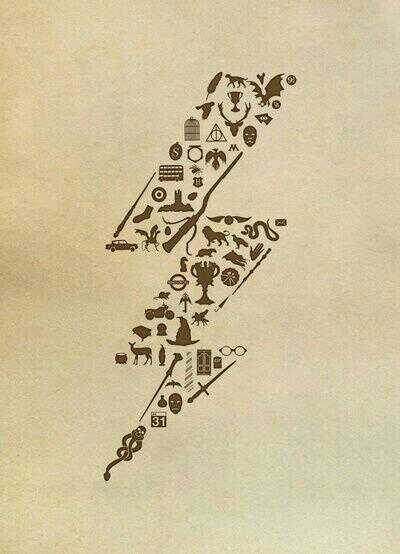
\includegraphics[scale=0.3]{harrypotter}
%	\caption{Test of figure.}
%	\label{centerOfMassDiagram}
%\end{figure}


%\begin{table}[H]
%	\centering
%	\begin{tabular}{|p{4.8cm}|p{2cm}|}
%		\hline%------------------------------------------------------------------------------------
%		\textbf{Characteristics}                 &  \textbf{Value} \unitWh{Unit}  \\
%		\hline%------------------------------------------------------------------------------------
%		Nominal output current                   &  5 \unitWh{A}  	\\
%		\hline%------------------------------------------------------------------------------------
%		Peak current (<20 s)                     &  15 \unitWh{A}	\\
%		\hline%------------------------------------------------------------------------------------
%		Current control PWM frequency 				   &  53,6 \unitWh{kHz}  \\
%		\hline%------------------------------------------------------------------------------------
%		Sample Rate of PI current controller     &  53,6 \unitWh{kHz}  \\
%		\hline%------------------------------------------------------------------------------------
%	\end{tabular}
%	\caption{Important parameters of the motor control board.}
%	\label{MotorControlBoardTable}
%\end{table}

%\begin{flalign}
%\eq{J_F \vec{\ddot{\theta}_F}} { -B_F \vec{\dot{\theta}_F} + \vec{l_F} \times (m_F\cdot \vec{g}) + \vec{l_w} \times \vec{F} - \vec{\tau_m} + B_w \vec{\dot{\theta}_w}} \unit{N\cdot m}
%\label{frameModelEq}
%\end{flalign}

%\begin{flalign}
%\eqOne{\tau_{m}[n]}{\num{-8,314} \cdot e_{\theta}[n]+ \num{7,422} \cdot e_{\theta}[n-1] + \num{8,3023} \cdot e_{\theta}[n-2] }
%\eqTwo{ - \num{7,434} \cdot e_{\theta}[n-3] + \num{1,382} \cdot \tau_{m}[n-1] - \num{0,3415} \cdot \tau_{m}[n-2] }
%\eqThree{- \num{0,001638} \cdot \tau_{m}[n-3]} \unit{N \cdot m} 
%\label{eq:discControllerDiffEq}
%\end{flalign}

\section{Method}
The methods presented in this section are constituted by the modelling of the system, the linearization of the obtained model and the design of the controllers.
\subsection{Model}
\begin{itemize}
\item Model - Drawing, equations, linear equations.
The quadcopter system is shown in Figure \ref{droneDiagram}. As it can bee seen, the system is modeled by using two coordinate frames. The inertial frame is utilized to describe the translational movement while the body frame is attached to the quadcopter and used to characterize its attitude behavior. In the figure, also the positive references for rotational and translational movements are depicted, as well as the main forces and torques acting on the quadcopter. 
\begin{figure}[H]
	\centering
	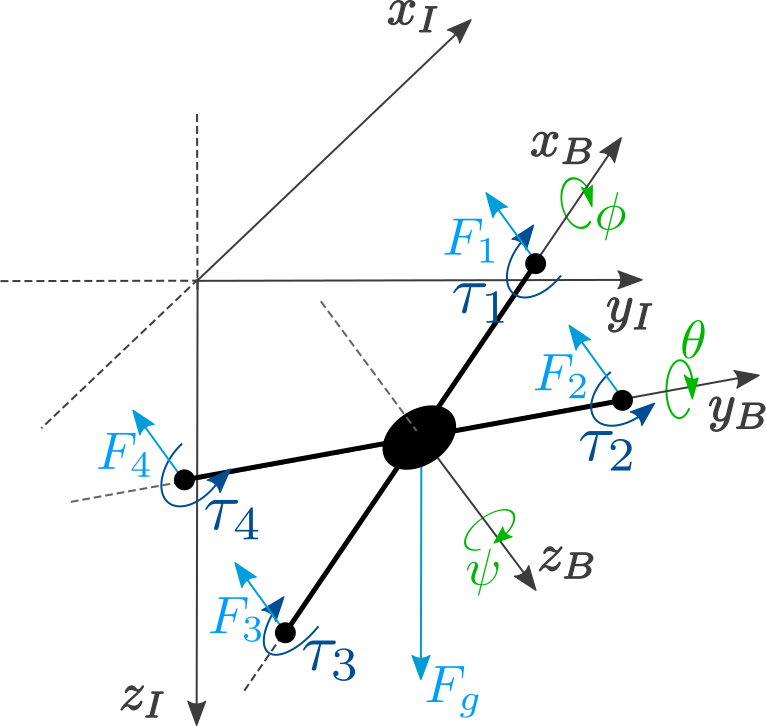
\includegraphics[scale=0.3]{droneDiagram}
	\caption{Quadcopter diagram showing the forces and torques acting on the system and the positive references chosen for rotations and translations in both Inertial and Body coordinate frames.}
	\label{droneDiagram}
\end{figure}
The forces generated in the propeller are easily explained in the Body coordinate frame. In order to represent them in the Inertial frame a rotation matrix is used. It is built considering a 123 rotation sequence. \textbf{SOURCE ROTATION  MATRIX}
 
The dynamic model of the quadcopter can be explain through three sets of equations. The first describes the motor and the propeller, the second presents the attitude response of the quadcopter and the third explains hos the translational variables of the system evolve with time.
\subsubsection{Motor and Propeller}
The four motors in the quadcopter generate the rotation required so the propeller creates the force that lifts the quadcopter. This force is called thrust force and can be modeled as proportional to the square of the motor rotational velocity. MAYBE SOURCE. The coefficient for this equation is called thrust coefficient and has been found by experiments.  
The rotation of the propellers also generates a torque on each motor due to drag between air and propeller. Drag torque is compensated in the quadcopter by having two of the motors turning in one direction and the two others in the opposite. It can also be described as proportional to the square of the velocity by terms of a drag coefficient that has also been obtained through tests.
Equation \ref{eq:thrustForce} and \ref{eq:dragTorque} show the expression for the thrust force and drag torque caused by the rotation of the propeller.
\begin{align}
	F&=k_{th}\omega^2\label{eq:thrustForce}\\
	\tau&=k_{d}\omega^2\label{eq:dragTorque}
\end{align}
\textbf{INCLUDE WHERE}\\
This equations are included in the attitude and translational models derived below.
\subsubsection{Attitude Model}
The attitude model equations are based on Newton Second Law for rotational movement and are represented in Equation \ref{eq:AngleEqVelocities1}, \ref{eq:AngleEqVelocities2} and \ref{eq:AngleEqVelocities3}. 
\begin{align}
	J_x\ddot{\phi}&=k_{th} (\omega^2_4-\omega^2_2)  L \label{eq:AngleEqVelocities1}\\
	J_y \ddot{\theta}&=k_{th} (\omega^2_1-\omega^2_3)  L \label{eq:AngleEqVelocities2} \\
	J_z\ddot{\psi}&=k_d (\omega^2_1-\omega^2_2+\omega^2_3-\omega^2_4)\label{eq:AngleEqVelocities3}
\end{align}
\textbf{INCLUDE WHERE}\\
%\begin{where}
%	\va{k_{th}}{is the thrust coefficients}{N\cdot s^2 \cdot rad^{-2}}
%	\va{k_d}{is the drag coefficients}{N \cdot m\cdot s^2 \cdot rad^{-2}}
%\end{where}
The expressions above state how the thrust force difference between motors 1 and 3 affects the roll angular acceleration, how that between motors 4 and 2 affects the pitch angle and how the yaw acceleration depends on the four motors by means of the drag torque generated on the propeller.  
\subsubsection{Translational Model}
The equations describing the response of the system along the x, y and z axes is derived from Newton's Second Law. The forces that act on the system are those from the propellers and the gravitational. These expressions are shown in Equation \ref{eq:AccelerationEqInertial1}, \ref{eq:AccelerationEqInertial2} and \ref{eq:AccelerationEqInertial3}. FIX EQUATIONS
\begin{flalign}
 	\eq{m\ddot{x}_I}{-k_{th}({\omega_1}^2+{\omega_2}^2+{\omega_3}^2+{\omega_4}^2)\sin(\theta)} \label{eq:AccelerationEqInertial1}\\
 	\eq{m\ddot{y}_I}{-k_{th}({\omega_1}^2+{\omega_2}^2+{\omega_3}^2+{\omega_4}^2)(-\sin(\phi))\cdot\cos(\theta)} \label{eq:AccelerationEqInertial2}\\
 	\eq{m\ddot{z}_I}{F_g-k_{th}({\omega_1}^2+{\omega_2}^2+{\omega_3}^2+{\omega_4}^2)\cos(\phi)\cdot\cos(\theta)}
 	\label{eq:AccelerationEqInertial3}
\end{flalign}
It is worth mentioning that, as the thrust forces always point in the negative z direction in the body coordinate frame, the accelerations in x and y directions in the inertial frame are zero as long as pitch and roll angles are 0.
\subsection{Linearization}
The linearization of the model equations has been developed following the first order Taylor approximation around an equilibrium point of the system. The chosen point is the hovering position and that implies that all variables have a value of zero, that is, the translational and attitude accelerations, velocities and positions. Choosing a zero acceleration equilibrium point along the Inertial z axis yields a equilibrium rotational speeds so that the necessary thrust is generated to compensate for the gravitational force.

The resulting equations for the attitude model after the linearization are shown in Equation \ref{eqAngleLin1}, \ref{eqAngleLin2} and \ref{eqAngleLin3}. 
\begin{flalign}
	J_x\Delta\ddot{\phi}   &= 2k_{th}L({\overline{\omega}_4} \Delta \omega_2-{\overline{\omega}_2} \Delta \omega_4)
	\label{eqAngleLin1} \\
	J_y\Delta\ddot{\theta} &= 2k_{th} L({\overline{\omega}_1} \Delta \omega_1-{\overline{\omega}_3} \Delta \omega_3) 
	\label{eqAngleLin2} \\
	J_z\Delta\ddot{\psi}   &= 2k_d({\overline{\omega}_1}\Delta \omega_1-{\overline{\omega}_2}\Delta \omega_2+{\overline{\omega}_3}\Delta \omega_3-{\overline{\omega}_4} \Delta \omega_4) \label{eqAngleLin3}
\end{flalign}
\textbf{INCLUDEWHERE}
%\begin{where}
%	\va{ \Delta\ddot{\phi}     } {is the change in roll angular acceleration from equilibrium}         { rad \cdot s^{-2} }
%	\va{ \Delta\ddot{\theta}   } {is the change in pitch angular acceleration from equilibrium}        { rad \cdot s^{-2} }
%	\va{ \Delta\ddot{\psi}     } {is the change in yaw angular acceleration from equilibrium}          { rad \cdot s^{-2} }
%	\va{ \overline{\omega}_i } {is the angular velocity of each motor in equilibrium}             { rad \cdot s^{-1} }
%	\va{ \Delta \omega_i       } {is the change in angular velocity from equilibrium of each motor} { rad \cdot s^{-1} }
%\end{where}
Similarly, the equations of the translational model are linearized. The result is shown in \ref{eq:TransLinearEquations1}, \ref{eq:TransLinearEquations2} and \ref{eq:TransLinearEquations3}. \textbf{FIX EQUATIONS}
\begin{flalign}
	m\cdot\Delta\ddot{x}_I &= -k_{th}({\overline{\omega}_1}^2+{\overline{\omega}_2}^2+{\overline{\omega}_3}^2+{\overline{\omega}_4}^2)\cos(\overline{\theta}) \Delta\theta \label{eq:TransLinearEquations1} \\
	m\cdot\Delta\ddot{y}_I &=  k_{th}({\overline{\omega}_1}^2+{\overline{\omega}_2}^2+{\overline{\omega}_3}^2+{\overline{\omega}_4}^2)\cos(\overline{\phi})\cos(\overline{\theta})\Delta\phi \label{eq:TransLinearEquations2}\\
	m\Delta\ddot{z}_I &= -2\textbf{ }k_{th}({\overline{\omega}_1}\Delta\omega_1+{\overline{\omega}_2}\Delta\omega_2+{\overline{\omega}_3}\Delta\omega_3+{\overline{\omega}_4}\Delta\omega_4)\cos(\overline{\phi})\cos(\overline{\theta})\label{eq:TransLinearEquations3}
\end{flalign} 
\textbf{INCLUDEWHERE}
%
%\begin{where}
%	\va{\Delta\ddot{x_I}  }{ is the change in linear acceleration from equilibrium in $x_I$ direction }{ m \cdot s^{-2} } \\
%	\va{\Delta\ddot{y_I}  }{ is the change in linear acceleration from equilibrium in $y_I$ direction }{ m \cdot s^{-2} } \\
%	\va{\Delta\ddot{z_I}  }{ is the change in linear acceleration from equilibrium in $z_I$ direction }{ m \cdot s^{-2} } \\
%	\va{\Delta \phi       }{ is the change in roll from equilibrium                          }{ rad            } \\
%	\va{\Delta \theta     }{ is the change in pitch from equilibrium                         }{ rad            } \\
%	\va{\Delta \psi       }{ is the change in yaw from equilibrium                           }{ rad            } \\
%	\va{\overline{\phi}   }{ is the roll in equilibrium                                      }{ rad            } \\
%	\va{\overline{\theta} }{ is the pitch in equilibrium                                     }{ rad            } \\
%	\va{\overline{\psi}   }{ is the yaw in equilibrium                                       }{ rad            }
%\end{where}
\subsection{Control}
The control of the system is divided into two control systems. One handles the attitude equations and the other controls the translational variables. 
\subsubsection{Attitude Controller}
The attitude controller for the quadcopter has been designed using a state space representation of the system. This helps handling the coupled angular response of the quadcopter.The chosen states for the system are the three angular positions and the three angular velocities. The input of the attitude system are the four motor rotational speeds and the output are the three angles roll, pitch and yaw. Below, the state vector, the input and the output are represented.
%
\begin{flalign}
	\vec{x}(t) = 
	\begin{bmatrix}
		\phi & \theta & \psi & \dot{\phi} &	\dot{\theta} & \dot{\psi} \\
	\end{bmatrix}	\nonumber
	^T
	\label{xVector}
\end{flalign}  
\begin{flalign}
	\vec{y}(t) = 
	\begin{bmatrix}
		\phi &	\theta & \psi \\
	\end{bmatrix}	\nonumber
	^T
	\label{yVector}
\end{flalign}
\begin{flalign}
	\vec{u}(t)= 
	\begin{bmatrix}
		\omega_1 & \omega_2 &	\omega_3 &	\omega_4 \\
	\end{bmatrix}\nonumber	
	^T
	\label{uVector}
\end{flalign}
%
The state space matrix representation is displayed in Equation \ref{xDotSS} and \ref{ySS}.
\begin{flalign}
	\vec{\dot{x}}(t)&=\vec{A} \cdot \vec{x}(t) + \vec{B} \cdot \vec{u}(t)
	\label{xDotSS} 
\end{flalign}
\begin{flalign}
	\vec{y}(t)&=\vec{C} \cdot \vec{x}(t) + \vec{D} \cdot \vec{u}(t)
	\label{ySS} 
\end{flalign}
\textbf{INCLUDEWHERE}
The values for the A, B, C and D matrices are obtained from the linearized attitude equations, yielding the matrices shown below. As D is a zero matrix, only A, B and C are shown.
\footnotesize
\begin{flalign}   \label{Amatrix}
	\vec{A}=
	\begin{bmatrix}
		\ 0 & 0 & 0 & 1 & 0 & 0     \ \ \ \\ 
		\ 0 & 0 & 0 & 0 & 1 & 0     \ \ \ \\ 
		\ 0 & 0 & 0 & 0 & 0 & 1     \ \ \ \\
		\ 0 & 0 & 0 & 0 & 0 & 0     \ \ \ \\ 
		\ 0 & 0 & 0 & 0 & 0 & 0     \ \ \ \\ 
		\ 0 & 0 & 0 & 0 & 0 & 0     \ \ \  		
	\end{bmatrix}\nonumber
\end{flalign} \label{Bmatrix}
\begin{flalign}
    \vec{B} =
	\begin{bmatrix}
		\ 0 & 0 & 0 & 0      \ \ \ \\ 
		\ 0 & 0 & 0 & 0      \ \ \ \\ 
		\ 0 & 0 & 0 & 0      \ \ \ \\
		\ 0 & \si{-\frac{2 \cdot k_{th} \cdot L \cdot \overline{\omega}_2}{J_x}} & 0 & \si{\frac{2 \cdot k_{th} \cdot L \cdot \overline{\omega}_4}{J_x}}      \ \ \ \\ 
		\ \si{\frac{2 \cdot k_{th} \cdot L \cdot \overline{\omega}_1}{J_y}} & 0 & \si{-\frac{2 \cdot k_{th} \cdot L \cdot \overline{\omega}_3}{J_y}} & 0      \ \ \ \\ 
		\ \frac{2 \cdot k_d \cdot {\overline{\omega}_1}}{J_z} & - \frac{2 \cdot k_d \cdot {\overline{\omega}_2}}{J_z} & \frac{2 \cdot k_d \cdot {\overline{\omega}_3}}{J_z} & - \frac{2 \cdot k_d \cdot {\overline{\omega}_4}}{J_z}      \ \ \ 		
	\end{bmatrix}\nonumber
\end{flalign}
\begin{flalign} \label{Cmatrix}
	\vec{C} =	 
	\begin{bmatrix}
		\ 1 & 0 & 0 & 0 & 0 & 0     \ \ \ \\ 
		\ 0 & 1 & 0 & 0 & 0 & 0     \ \ \ \\ 
		\ 0 & 0 & 1 & 0 & 0 & 0     \ \ \ 		
	\end{bmatrix}\nonumber
\end{flalign}
\normalsize
The controller designed is depicted in the block diagram shown in Figure \ref{attitudeControlDiagram}.
\begin{figure}[H]
	\centering
	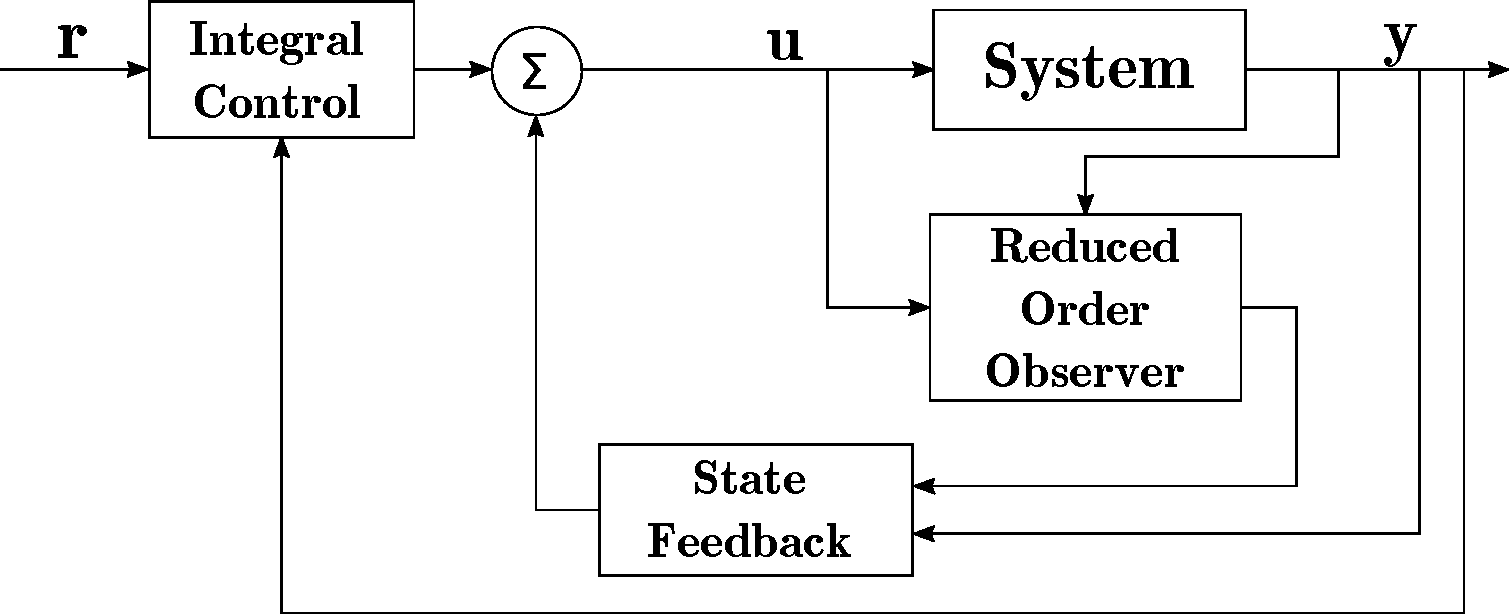
\includegraphics[scale=0.3]{AttitudeControlDiagram}
	\caption{Control structure for regulating the attitude response of the quadcopter. It includes the state feedback, the reduced order observer and the integral term.}
	\label{attitudeControlDiagram}
\end{figure}
\subsubsection{Translational Controller}
\item Controller - Diagram of controller.
	\item Angle controller - include observer, linear controller.
\item Network effect on the system - Analysis of delay in the system.
\end{itemize}
\section{Results}
Simulation vs. reality. \\
%Design a setup that allows a nice measurement of reality - yet to be done\\
Comment on the results and how that correlates with reality, without discussing possible issues or improvements.

\section{Discussion}
Discussing possible issues or improvements of the above results.

\section{Conclusion}
Summary - what we want the reader to remember.
\section*{Acknowledgment}
Henrik XXXXX, associated professor at Aalborg University \\
Christoffer Sloth, associated professor at Aalborg University

% trigger a \newpage just before the given reference
% number - used to balance the columns on the last page
% adjust value as needed - may need to be readjusted if
% the document is modified later
%\IEEEtriggeratref{8}
% The "triggered" command can be changed if desired:
%\IEEEtriggercmd{\enlargethispage{-5in}}

% references section

% can use a bibliography generated by BibTeX as a .bbl file
% BibTeX documentation can be easily obtained at:
% http://mirror.ctan.org/biblio/bibtex/contrib/doc/
% The IEEEtran BibTeX style support page is at:
% http://www.michaelshell.org/tex/ieeetran/bibtex/
%\bibliographystyle{IEEEtran}
\printbibliography
% argument is your BibTeX string definitions and bibliography database(s)
%\bibliography{setup/bibliography.bbl}
%
% <OR> manually copy in the resultant .bbl file
% set second argument of \begin to the number of references
% (used to reserve space for the reference number labels box)

	%\begin{thebibliography}{}	
	%%\bibitem{IEEEhowto:kopka}
	%%H.~Kopka and P.~W. Daly, \emph{A Guide to \LaTeX}, 3rd~ed.\hskip 1em plus
	%%  0.5em minus 0.4em\relax Harlow, England: Addison-Wesley, 1999.
	%
	%\end{thebibliography}

% that's all folks
\end{document}

